\section{Partie pratique – création d’un programme KEYENCE} 
\noindent Dans ce labo, vous devrez créer un programme qui permette de : 
\begin{itemize}
  \item calculer et corriger la distorsion de la caméra,
  \item mesurer la longueur et la hauteur de différents objets,
  \item afficher les résultats à l’écran.
\end{itemize}
\vspace{0.3cm}

\noindent
\begin{minipage}[c]{\textwidth}
  \centering
  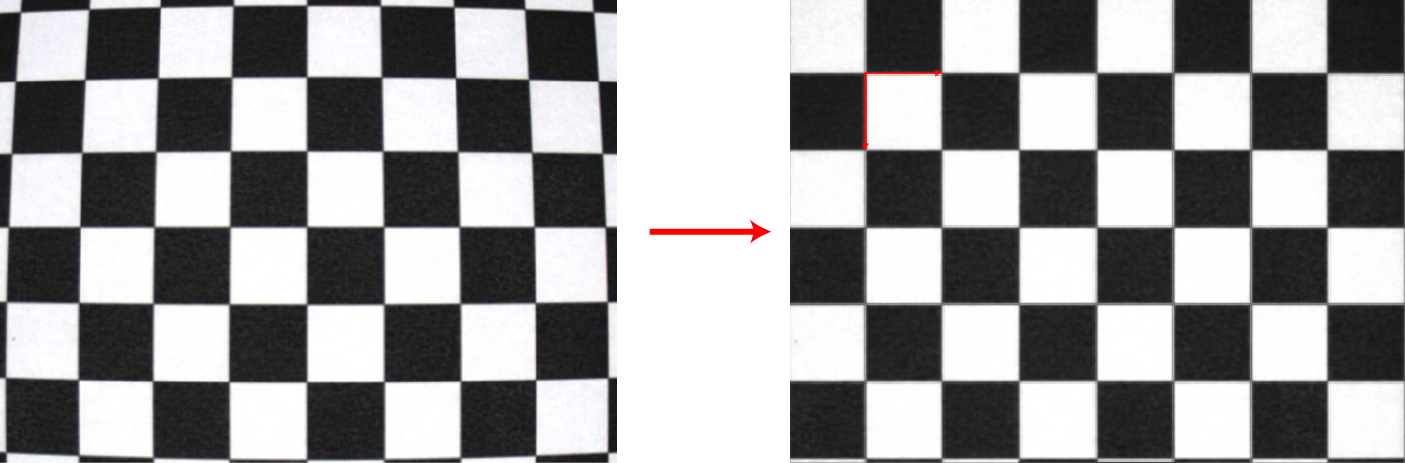
\includegraphics[width=16cm, height=10cm, keepaspectratio]{addOns/LaboCalib_Practical_chessboard.png}
  \captionof{figure}{\textit{Résultats de la calibration sur le damier de calibration}}
  \label{fig.Image_RefImagesSwitch}
\end{minipage}\\
\vspace{0.3cm}

\noindent
\begin{minipage}[c]{\textwidth}
  \centering
  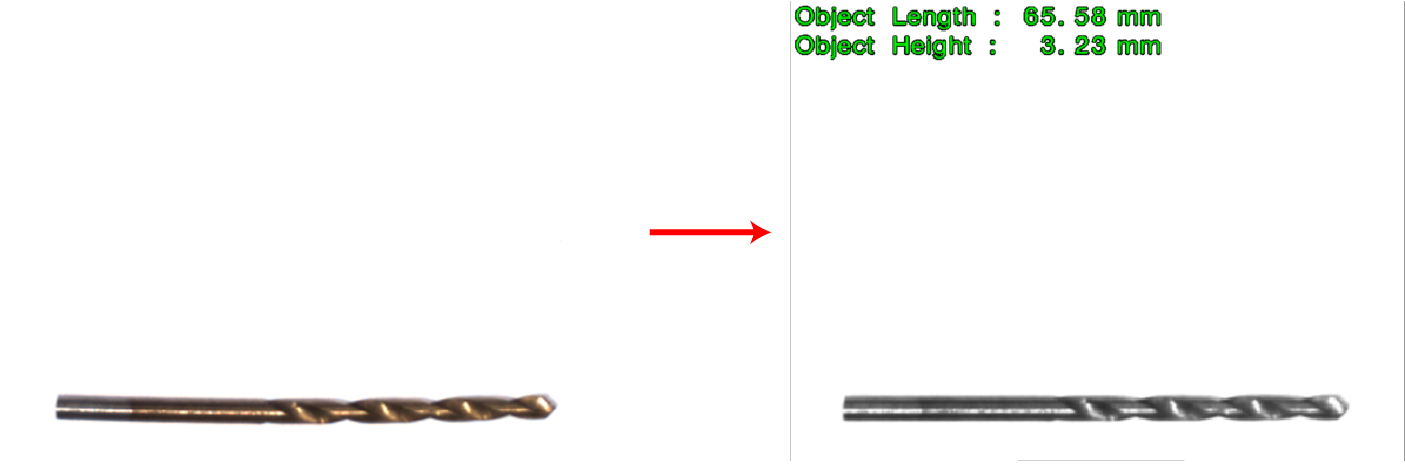
\includegraphics[width=16cm, height=10cm, keepaspectratio]{addOns/LaboCalib_Practical_object.png}
  \captionof{figure}{\textit{Entrée et Sortie+affichage du programme demandé}}
  \label{fig.Image_RefImagesSwitch}
\end{minipage}\\
\vspace{0.3cm}

Une partie des blocs de fonctions seront présentés durant le laboratoire, mais en cas de doutes/questions plus approfondis, référez-vous à la documentation fournie par KEYENCE 
\begin{center}
\textit{KEYENCE XG-X VisionEditor Reference Manual}
\end{center}
\noindent qui contient toutes les fonctions et leur paramétrage.

\newpage
\subsection{Résultats observés}
Reportez ci-dessous les dimensions des objets que vous avez mesurées sur les différentes images grâce à votre programme :\\
\begin{table}[ht]
  \renewcommand{\arraystretch}{3}
  \newcolumntype{x}[1]{>{\centering\let\newline\\\arraybackslash\hspace{0pt}}p{#1}}
  \center
  \begin{tabular}{|c|x{3cm}|x{3cm}|x{3cm}|}
    \hline
    \multicolumn{2}{|c|}{\large{\textbf{Objets}}} & \large{\textbf{Hauteur [mm]}} & \large{\textbf{Largeur [mm]}} \\
    \hline
    \multirow{4}{0.3cm}{\rotatebox[origin=c]{90}{\large{\textbf{Objet 1}}}} & \textit{Théorique}
      & {\LARGE 3} & {\LARGE 65.5} \\
    & image 1 & & \\
    & image 2 & & \\
    & image 3 & & \\
    \hline  
    \multirow{4}{0.3cm}{\rotatebox[origin=c]{90}{\large{\textbf{Objet 2}}}} & \textit{Théorique}
      & {\LARGE 35.5} & {\LARGE 8.5} \\
    & image1 & & \\
    & image2 & & \\
    \hline
  \end{tabular}
  \caption{Résultats mesurés avec votre programme}
\end{table}

\vspace{0.3cm}
